% defer/refcnt.tex

\section{Reference Counting}
\label{sec:defer:Reference Counting}

{ \scriptsize
\begin{verbbox}
 1 struct route_entry {
 2   atomic_t re_refcnt;
 3   struct route_entry *re_next;
 4   unsigned long addr;
 5   unsigned long iface;
 6   int re_freed;
 7 };
 8 struct route_entry route_list;
 9 DEFINE_SPINLOCK(routelock);
10
11 static void re_free(struct route_entry *rep)
12 {
13   ACCESS_ONCE(rep->re_freed) = 1;
14   free(rep);
15 }
16
17 unsigned long route_lookup(unsigned long addr)
18 {
19   int old;
20   int new;
21   struct route_entry *rep;
22   struct route_entry **repp;
23   unsigned long ret;
24
25 retry:
26   repp = &route_list.re_next;
27   rep = NULL;
28   do {
29     if (rep &&
30         atomic_dec_and_test(&rep->re_refcnt))
31       re_free(rep);
32     rep = ACCESS_ONCE(*repp);
33     if (rep == NULL)
34       return ULONG_MAX;
35     do {
36       if (ACCESS_ONCE(rep->re_freed))
37         abort();
38       old = atomic_read(&rep->re_refcnt);
39       if (old <= 0)
40         goto retry;
41       new = old + 1;
42     } while (atomic_cmpxchg(&rep->re_refcnt,
43                             old, new) != old);
44     repp = &rep->re_next;
45   } while (rep->addr != addr);
46   ret = rep->iface;
47   if (atomic_dec_and_test(&rep->re_refcnt))
48     re_free(rep);
49   return ret;
50 }
\end{verbbox}
}
\begin{figure}[bp]
\centering
\theverbbox
\caption{Reference-Counted Pre-BSD Routing Table Lookup}
\label{fig:defer:Reference-Counted Pre-BSD Routing Table Lookup}
\end{figure}

{ \scriptsize
\begin{verbbox}
 1 int route_add(unsigned long addr,
 2               unsigned long interface)
 3 {
 4   struct route_entry *rep;
 5
 6   rep = malloc(sizeof(*rep));
 7   if (!rep)
 8     return -ENOMEM;
 9   atomic_set(&rep->re_refcnt, 1);
10   rep->addr = addr;
11   rep->iface = interface;
12   spin_lock(&routelock);
13   rep->re_next = route_list.re_next;
14   rep->re_freed = 0;
15   route_list.re_next = rep;
16   spin_unlock(&routelock);
17   return 0;
18 }
19
20 int route_del(unsigned long addr)
21 {
22   struct route_entry *rep;
23   struct route_entry **repp;
24
25   spin_lock(&routelock);
26   repp = &route_list.re_next;
27   for (;;) {
28     rep = *repp;
29     if (rep == NULL)
30       break;
31     if (rep->addr == addr) {
32       *repp = rep->re_next;
33       spin_unlock(&routelock);
34       if (atomic_dec_and_test(&rep->re_refcnt))
35         re_free(rep);
36       return 0;
37     }
38     repp = &rep->re_next;
39   }
40   spin_unlock(&routelock);
41   return -ENOENT;
42 }
\end{verbbox}
}
\begin{figure}[bp]
\centering
\theverbbox
\caption{Reference-Counted Pre-BSD Routing Table Add/Delete}
\label{fig:defer:Reference-Counted Pre-BSD Routing Table Add/Delete}
\end{figure}

\begin{figure}[tb]
\begin{center}
\resizebox{2.5in}{!}{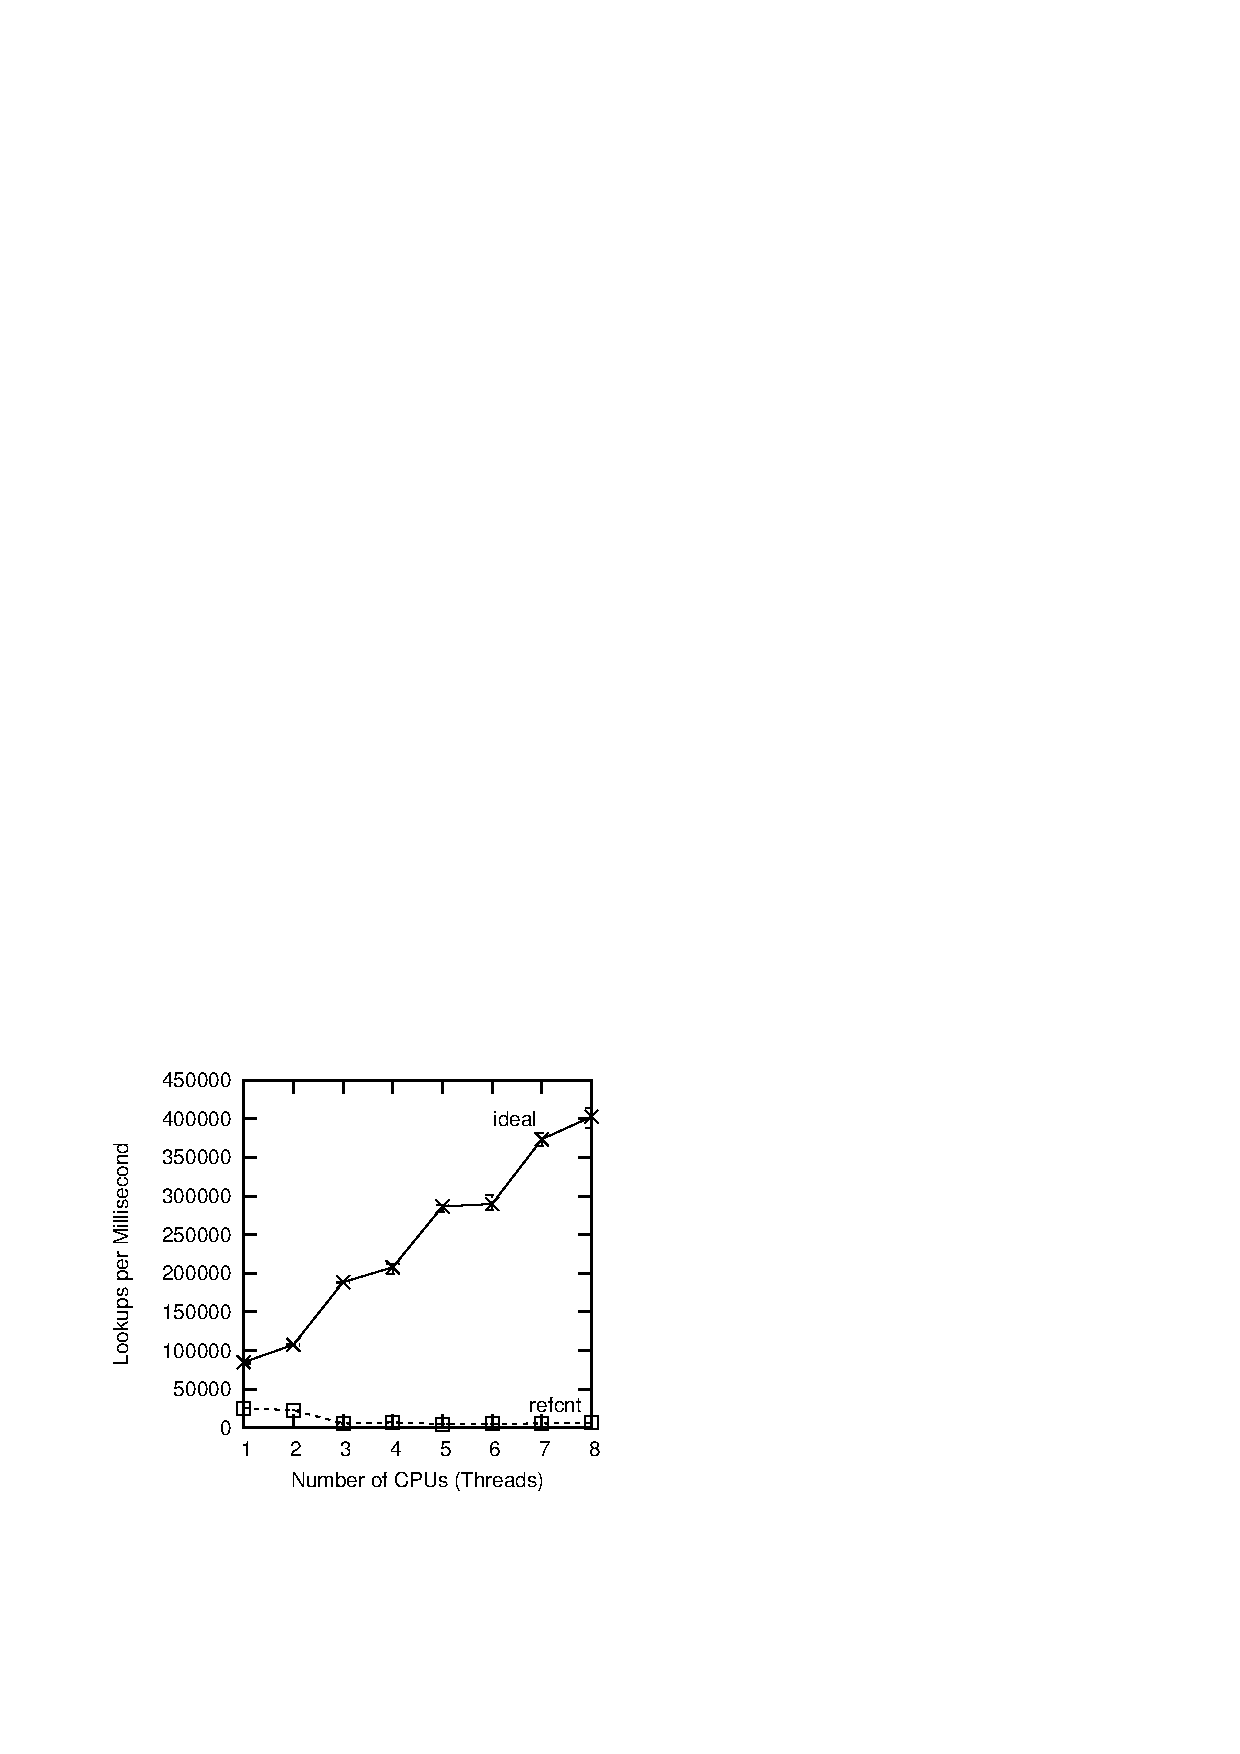
\includegraphics{CodeSamples/defer/data/paulmck.2016/perf-refcnt}}
\end{center}
\caption{Pre-BSD Routing Table Protected by Reference Counting}
\label{fig:defer:Pre-BSD Routing Table Protected by Reference Counting}
\end{figure}

레퍼런스 카운팅은 하나의 오브젝트에 대해 이 오브젝트가 너무 이르게 메모리
해제되는 일을 방지하기 위해 존재하는 레퍼런스의 횟수를 셉니다.


이는 컨셉적으로는 간단한 테크닉이지만, 실제 자세한 내용 안에 많은 악마들이
숨어있습니다.
일단, 이 오브젝트가 준비되지 않은 상황에서 폐기되더라도 문제가 없다고 하면,
레퍼런스 카운터를 둘 이유 자체가 없을 겁니다.
하지만 이 오브젝트가 폐기될 수 있다면, 어떻게 하면 오브젝트가 레퍼런스 획득
처리과정 중에 폐기되는 것을 막을 수 있을까요?

이 질문에는 많은 답변이 존재할 수 있는데, 다음의 것들을 포함합니다:
\iffalse

Reference counting tracks the number of references
to a given object in order to prevent that object from being prematurely
freed.


Although this is a conceptually simple technique, many devils hide in
the details.
After all, if the object was not subject to premature disposal,
there would be no need for the reference counter in the first place.
But if the object can be disposed of, what prevents disposal during
the reference-acquisition process itself?

There are a number of possible answers to this question, including:
\fi

\begin{enumerate}
\item	레퍼런스 카운트를 조정하는 동안 해당 오브젝트의 밖에 존재하는 락을 잡고
	있어야만 합니다.
\item	이 오브젝트는 0 이 아닌 값을 갖는 레퍼런스 카운트를 가지고 생성되고,
	레퍼런스 카운터의 현재 값이 0이 아닐 때에만 새로운 레퍼런스가 얻어질 수
	있습니다.
	어떤 쓰레드가 어떤 오브젝트에 레퍼런스를 가지고 있지 않다면, 해당
	쓰레드는 이미 레퍼런스를 가지고 있는 다른 쓰레드의 도움으로 레퍼런스를
	하나 얻을 수 있을 겁니다.
\item	오브젝트의 존재 보장이 제공되어서, 어떤 다른 것들이 레퍼런스를 얻으려
	시도하는 동안은 메모리 해제되는 것을 방지해 줍니다.
	존재 보장은 많은 경우 자동화된 가비지 콜렉터에 의해 제공되기도 하고,
	Section~\ref{sec:defer:Read-Copy Update (RCU)} 에서 보게 될테지만, RCU
	에 의해 제공되기도 합니다.
\item	타입 안전성 보장이 해당 오브젝트에 제공됩니다.
	레퍼런스가 획득될 때마다 추가적인 타입 안정성 체크가 반드시 이루어져야
	합니다.
	타입 안정성 보장은 특수 목적의 메모리 할당자를 통해 제공될 수 있는데,
	예를 들면 리눅스 커널의 \co{SLAB_DESTROY_BY_RCU} 기능과 같은 것으로,
	Section~\ref{sec:defer:Read-Copy Update (RCU)} 에서 다루어질 겁니다.
\iffalse

\item	A lock residing outside of the object must be held while
	manipulating the reference count.
\item	The object is created with a non-zero reference count, and new
	references may be acquired only when the current value of
	the reference counter is non-zero.
	If a thread does not have a reference to a given object,
	it may obtain one with the help of another thread that
	already has a reference.
\item	An existence guarantee is provided for the object, preventing
	it from being freed while some other
	entity might be attempting to acquire a reference.
	Existence guarantees are often provided by automatic
	garbage collectors, and, as will be seen in
	Section~\ref{sec:defer:Read-Copy Update (RCU)}, by RCU.
\item	A type-safety guarantee is provided for the object.
	An additional identity check must be performed once
	the reference is acquired.
	Type-safety guarantees can be provided by special-purpose
	memory allocators, for example, by the
	\co{SLAB_DESTROY_BY_RCU} feature within the Linux kernel,
	as will be seen in Section~\ref{sec:defer:Read-Copy Update (RCU)}.
\fi
\end{enumerate}

물론, 존재 보장을 제공하는 메커니즘은 모두 그 정의에 의해 타입 안정성 보장 역시
제공합니다.
따라서 이 섹션은 마지막의 두 답을 RCU 의 규정 아래에서 함께 묶어서 다뤄서,
레퍼런스 획득 보호의 세가지 카테고리만을 다루도록 하겠습니다: 레퍼런스 카운팅,
순차적 락킹, 그리고 RCU.
\iffalse

Of course, any mechanism that provides existence guarantees
by definition also provides type-safety guarantees.
This section will therefore group the last two answers together under the
rubric of RCU, leaving us with three general categories of
reference-acquisition protection: Reference counting, sequence
locking, and RCU.
\fi

\QuickQuiz{}
	레퍼런스 획득을 레퍼런스 카운터의 값이 0이 아닐 때에만 레퍼런스를
	획득하는 간단한 compare-and-swap 오퍼레이션을 사용해서 구현하는 건
	어떤가요?
	\iffalse

	Why not implement reference-acquisition using
	a simple compare-and-swap operation that only
	acquires a reference if the reference counter is
	non-zero?
	\fi
\QuickQuizAnswer{
	이 방법은 마지막 레퍼런스의 해제와 새로운 레퍼런스의 획득 사이의 경주를
	해결할 수 있긴 하지만, 데이터 구조체가 메모리 해제되고 그 영역이 어떤
	전혀 다른 타입의 구조체로 재할당 되는 것을 막는데에는 어떤 일도 해주지
	않습니다.
	``간단한 compare-and-swap 오퍼레이션'' 이 다른 타입의 구조체에
	적용된다면 정의되지 않은 결과를 낼 확률이 높습니다.

	요약해서, compare-and-swap 과 같은 어토믹 오퍼레이션들의 사용은 분명히
	타입 안정성이나 존재 보장을 필요로 합니다.
	\iffalse

	Although this can resolve the race between the release of
	the last reference and acquisition of a new reference,
	it does absolutely nothing to prevent the data structure
	from being freed and reallocated, possibly as some completely
	different type of structure.
	It is quite likely that the ``simple compare-and-swap
	operation'' would give undefined results if applied to the
	differently typed structure.

	In short, use of atomic operations such as compare-and-swap
	absolutely requires either type-safety or existence guarantees.
	\fi
} \QuickQuizEnd

\begin{table}
\centering
\begin{tabular}{l||c|c|c}
	& \multicolumn{3}{c}{Release Synchronization} \\
	\cline{2-4}
	Acquisition     &         & Reference &     \\
	Synchronization & Locking & Counting  & RCU \\
	\hline
	\hline
	Locking		& -	  & CAM	      & CA  \\
	\hline
	Reference	& A	  & AM	      & A   \\
	Counting	&  	  &   	      &     \\
	\hline
	RCU		& CA	  & MCA	      & CA  \\
\end{tabular}
\caption{Reference Counting and Synchronization Mechanisms}
\label{tab:defer:Reference Counting and Synchronization Mechanisms}
\end{table}

레퍼런스 카운팅의 핵심 이슈는 레퍼런스의 획득과 객체의 메모리 해제 사이에서의
동기화라는 점을 놓고 보면,
Table~\ref{tab:defer:Reference Counting and Synchronization Mechanisms} 에
보여진 것과 같이 아홉개의 메커니즘들의 조합이 존재함을 알 수 있습니다.
이 표는 레퍼런스 카운팅 메커니즘을 다음과 같이 넓은 카테고리들로 나눕니다:
\iffalse

Given that the key reference-counting issue
is synchronization between acquisition
of a reference and freeing of the object, we have nine possible
combinations of mechanisms, as shown in
Table~\ref{tab:defer:Reference Counting and Synchronization Mechanisms}.
This table
divides reference-counting mechanisms into the following broad categories:
\fi
\begin{enumerate}
\item	어토믹 오퍼레이션들이나 메모리 배리어, 또는 메모리 정렬 제약 없이
	이루어지는 간단한 카운팅 \makebox{(``-'')}.
\item	메모리 배리어 없이 하는 어토믹하게 하는 카운팅 (``A'').
\item	레퍼런스 해제에만 메모리 배리어를 사용하며 어토믹하게 하는 카운팅
	(``AM'').
\item	레퍼런스 해제에는 메모리 배리어를 사용하고 어토믹한 레퍼런스 획득에
	검사를 결합한 어토믹한 카운팅 (``CAM'').
\item	어토믹한 레퍼런스 획득 오퍼레이션에 검사를 결합한 어토믹 카운팅
	(``CA'').
\item	레퍼런스 해제와 획득 모두에 메모리 배리어를 사용하며 어토믹한 레퍼런스
	획득에 검사를 결합한 어토믹한 카운팅 (``MCA'').
\iffalse

\item	Simple counting with neither atomic operations, memory
	barriers, nor alignment constraints \makebox{(``-'')}.
\item	Atomic counting without memory barriers (``A'').
\item	Atomic counting, with memory barriers required only on release
	(``AM'').
\item	Atomic counting with a check combined with the atomic acquisition
	operation, and with memory barriers required only on release
	(``CAM'').
\item	Atomic counting with a check combined with the atomic acquisition
	operation (``CA'').
\item	Atomic counting with a check combined with the atomic acquisition
	operation, and with memory barriers also required on acquisition
	(``MCA'').
\fi
\end{enumerate}
하지만, 리눅스 커널의 값을 리턴하는 모든 어토믹 오퍼레이션들은 메모리 배리어를
포함하도록 되어 있기 때문에,\footnote{
	\co{atomic_read()} 와 \co{ATOMIC_INIT()} 는 이 규칙의 예외입니다.}
모든 레퍼런스 해제 오퍼레이션들은 메모리 배리어들을 내포하고 있고, 모든 검사를
하는 레퍼런스 획득 오퍼레이션들 역시 메모리 배리어들을 포함하고 있습니다.
따라서, ``CA'' 와 ``MCA'' 케이스는 ``CAM'' 과 동일해서 실제로는 앞의 네가지
경우만 존재합니다:
\makebox{``-''}, ``A'', ``AM'', 그리고 ``CAM''.
레퍼런스 카운팅을 지원하는 리눅스의 도구들은
Section~\ref{sec:defer:Linux Primitives Supporting Reference Counting} 에 나와
있습니다.
뒤의 섹션들은 레퍼런스 획득과 해제가 매우 빈번하게 이루어지고 레퍼런스 카운트가
0인지의 검사가 매우 가끔씩 이루어질 때 성능을 개선할 수 있는 최적화들을
인용합니다.
\iffalse

However, because all Linux-kernel atomic operations that return a
value are defined to contain memory barriers,\footnote{
	With \co{atomic_read()} and \co{ATOMIC_INIT()} being the
	exceptions that prove the rule.}
all release operations
contain memory barriers, and all checked acquisition operations also
contain memory barriers.
Therefore, cases ``CA'' and ``MCA'' are equivalent to ``CAM'', so that
there are sections below for only the first four cases:
\makebox{``-''}, ``A'', ``AM'', and ``CAM''.
The Linux primitives that support reference counting are presented in
Section~\ref{sec:defer:Linux Primitives Supporting Reference Counting}.
Later sections cite optimizations that can improve performance
if reference acquisition and release is very frequent, and the
reference count need be checked for zero only very rarely.
\fi

\subsection{Implementation of Reference-Counting Categories}
\label{sec:defer:Implementation of Reference-Counting Categories}

락킹을 보호화는 간단한 카운팅 (\makebox{``-''}) 은
Section~\ref{sec:defer:Simple Counting} 에서,
메모리 배리어 없이 하는 어토믹한 카운팅 (``A'') 는
Section~\ref{sec:defer:Atomic Counting} 에서 설명되고
획득 시에의 메모리 배리어와 함께 사용되는 어토믹한 카운팅 (``AM'') 은
Section~\ref{sec:defer:Atomic Counting With Release Memory Barrier} 에서
설명되며, 검사와 해제시의 메모리 배리어를 사용하는 어토믹한 카운팅 (``CAM'') 은
Section~\ref{sec:defer:Atomic Counting With Check and Release Memory Barrier}
에서 설명됩니다.
\iffalse

Simple counting protected by locking (\makebox{``-''}) is described in
Section~\ref{sec:defer:Simple Counting},
atomic counting with no memory barriers (``A'') is described in
Section~\ref{sec:defer:Atomic Counting}
atomic counting with acquisition memory barrier (``AM'') is described in
Section~\ref{sec:defer:Atomic Counting With Release Memory Barrier},
and
atomic counting with check and release memory barrier (``CAM'') is described in
Section~\ref{sec:defer:Atomic Counting With Check and Release Memory Barrier}.
\fi

\subsubsection{Simple Counting}
\label{sec:defer:Simple Counting}

레퍼런스 획득과 해제가 모두 같은 락으로 보호된다면 어토믹 오퍼레이션도 메모리
배리어도 사용하지 않는 간단한 카운팅 방법이 레퍼런스 카운터로 사용될 수
있습니다.
이 경우, 레퍼런스 카운트 그 자체는 어토믹하지 않게 조정됨이 분명한데, 락은 모든
필요한 배타성, 메모리 배리어, 어토믹 오퍼레이션, 그리고 컴파일러 최적화의
방지를 제공하기 때문입니다.
이 방법은 레퍼런스 카운트 외에도 다른 오퍼레이션들을 보호하는데 락이 필요하지만
오브젝트로의 레퍼런스는 그 락이 해제된 이후에도 잡혀져 있어야 하는 경우에
사용되는 방법입니다.
Figure~\ref{fig:defer:Simple Reference-Count API} 는 간단한 어토믹하지 않은
레퍼런스 카운팅을 구현하는데 사용될 수도 있는 간단한 API 를 보입니다 -- 간단한
레퍼런스 카운팅은 거의 항상 공개된 코드이지만요.
\iffalse

Simple counting, with neither atomic operations nor memory barriers,
can be used when the reference-counter acquisition and release are
both protected by the same lock.
In this case, it should be clear that the reference count itself
may be manipulated non-atomically, because the lock provides any
necessary exclusion, memory barriers, atomic instructions, and disabling
of compiler optimizations.
This is the method of choice when the lock is required to protect
other operations in addition to the reference count, but where
a reference to the object must be held after the lock is released.
Figure~\ref{fig:defer:Simple Reference-Count API} shows a simple
API that might be used to implement simple non-atomic reference
counting -- although simple reference counting is almost always
open-coded instead.
\fi

{ \scriptsize
\begin{verbbox}
  1 struct sref {
  2   int refcount;
  3 };
  4
  5 void sref_init(struct sref *sref)
  6 {
  7   sref->refcount = 1;
  8 }
  9
 10 void sref_get(struct sref *sref)
 11 {
 12   sref->refcount++;
 13 }
 14
 15 int sref_put(struct sref *sref,
 16              void (*release)(struct sref *sref))
 17 {
 18   WARN_ON(release == NULL);
 19   WARN_ON(release == (void (*)(struct sref *))kfree);
 20
 21   if (--sref->refcount == 0) {
 22     release(sref);
 23     return 1;
 24   }
 25   return 0;
 26 }
\end{verbbox}
}
\begin{figure}[htbp]
\centering
\theverbbox
\caption{Simple Reference-Count API}
\label{fig:defer:Simple Reference-Count API}
\end{figure}

\subsubsection{Atomic Counting}
\label{sec:defer:Atomic Counting}

간단한 어토믹 카운팅은 레퍼런스를 획득하려는 CPU 는 반드시 레퍼런스를 이미
가지고 있어야 하는 경우에 사용될 수 있습니다.
이런 형태는 하나의 CPU 가 혼자 사용하기 위해 오브젝트를 생성하지만, 나중에 다른
CPU 나 task, 타이머 핸들러, 또는 I/O 완료 핸들러 등에게도 이 오브젝트를 접근할
수 있도록 해야 할 때 사용됩니다.
이 오브젝트를 넘겨주는 CPU 는 받는 쪽을 대신해서 먼저 새로운 레퍼런스를
얻어야만 합니다.
리눅스 커널에서는 \co{kref} 도구가 이런 형태의 레퍼런스 카운팅을 구현하기 위해
사용되는데,
Figure~\ref{fig:defer:Linux Kernel kref API} 에 나타나 있습니다.
\iffalse

Simple atomic counting may be used in cases where any CPU acquiring
a reference must already hold a reference.
This style is used when a single CPU creates an object for its
own private use, but must allow other CPU, tasks, timer handlers,
or I/O completion handlers that it later spawns to also access this object.
Any CPU that hands the object off must first acquire a new reference
on behalf of the recipient object.
In the Linux kernel, the \co{kref} primitives are used to implement
this style of reference counting, as shown in
Figure~\ref{fig:defer:Linux Kernel kref API}.
\fi

어토믹 카운팅이 필요한 이유는 모든 레퍼런스 카운트 오퍼레이션을 보호하는데
락킹이 사용되지 않기 때문인데, 이 말은 두개의 다른 CPU 들이 동시에 레퍼런스
카운트를 조정할 수도 있다는 뜻입니다.
평범한 값 증가와 감소 오퍼레이션이 사용되었다면, 이 두개의 CPU 들은 둘 다
레퍼런스 카운트를 동시에 읽어들여와서는 아마도 둘 다 ``3'' 이라는 값을 얻어올
수 있을 겁니다.
만약 둘 다 그 값을 증가시킨다면 둘 다 ``4'' 라는 값을 얻을 것이고, 둘은 이 값을
카운터에 다시 저장하려 할 것입니다.
카운터의 새로운 값은 그게 아니라 ``5'' 여야 하므로, 두개의 증가 연산 중 하나는
사라진 셈입니다.
따라서, 카운터 증가와 감소 두 경우 모두에 어토믹 오퍼레이션이 사용되어야만
합니다.
\iffalse

Atomic counting is required
because locking is not used to protect all reference-count operations,
which means that it is possible for two different CPUs to concurrently
manipulate the reference count.
If normal increment and decrement were used, a pair of CPUs might both
fetch the reference count concurrently, perhaps both obtaining
the value ``3''.
If both of them increment their value, they will both obtain ``4'',
and both will store this value back into the counter.
Since the new value of the counter should instead be ``5'', one
of the two increments has been lost.
Therefore, atomic operations must be used both for counter increments
and for counter decrements.
\fi

메모리 해제가 락킹이나 RCU 로 보호되고 있다면 메모리 배리어는 필요치
\emph{않습니다만}, 서로 다른 이유로 인한 것입니다.
락킹의 경우, 락들은 모든 필요한 메모리 배리어를 제공하고 (그리고 컴파일러
최적화를 방지합니다), 이 락들은 또한 동시에 수행되는 해제 작업들을 방지합니다.
RCU 의 경우, 메모리 정리는 모든 동시에 수행중인 RCU read-side 크리티컬 섹션들이
완료된 후로 미뤄져야 하고, 모든 필요한 메모리 배리어들이나 컴파일러 최적화의
제거는 RCU 기반 구조에서 제공되어질 겁니다.
따라서, 두개의 CPU 들이 마지막 두개의 레퍼런스들을 동시에 메모리에서
해제시키면, 실제 메모리 정리는 두 CPU 가 모두 RCU read-side 크리티컬 섹션을
종료한 이후로 미뤄질 겁니다.
\iffalse

If releases are guarded by locking or RCU,
memory barriers are \emph{not} required, but for different reasons.
In the case of locking, the locks provide any needed memory barriers
(and disabling of compiler optimizations), and the locks also
prevent a pair of releases from running concurrently.
In the case of RCU, cleanup must be deferred until all currently
executing RCU read-side critical sections have completed, and
any needed memory barriers or disabling of compiler optimizations
will be provided by the RCU infrastructure.
Therefore, if two CPUs release the final two references concurrently,
the actual cleanup will be deferred until both CPUs exit their
RCU read-side critical sections.
\fi

\QuickQuiz{}
	한 CPU 가 마지막 레퍼런스를 해제한 직후에 다른 CPU 가 레퍼런스를
	획득하는 경우에 대해서는 왜 보호가 필요치 않나요?
	\iffalse

	Why isn't it necessary to guard against cases where one CPU
	acquires a reference just after another CPU releases the last
	reference?
	\fi
\QuickQuizAnswer{
	CPU 는 다른 레퍼런스를 정상적으로 획득하기 위해서는 이미 레퍼런스를
	가지고 있어야 하기 때문입니다.
	따라서, 한 CPU 가 마지막 레퍼런스를 해제한다면, 새로운 레퍼런스를
	획득할 수 있도록 허용된 CPU 는 존재하지 않습니다.
	이와 똑같은 이유로 Figure~\ref{fig:defer:Linux Kernel kref API} 의
	line~22 에서의 어토믹하지 않은 검사가 가능합니다.
	\iffalse

	Because a CPU must already hold a reference in order
	to legally acquire another reference.
	Therefore, if one CPU releases the last reference,
	there cannot possibly be any CPU that is permitted
	to acquire a new reference.
	This same fact allows the non-atomic check in line~22
	of Figure~\ref{fig:defer:Linux Kernel kref API}.
	\fi
} \QuickQuizEnd

{ \scriptsize
\begin{verbbox}
  1 struct kref {
  2   atomic_t refcount;
  3 };
  4 
  5 void kref_init(struct kref *kref)
  6 {
  7   atomic_set(&kref->refcount, 1);
  8 }
  9 
 10 void kref_get(struct kref *kref)
 11 {
 12   WARN_ON(!atomic_read(&kref->refcount));
 13   atomic_inc(&kref->refcount);
 14 }
 15 
 16 static inline int
 17 kref_sub(struct kref *kref, unsigned int count,
 18          void (*release)(struct kref *kref))
 19 {
 20   WARN_ON(release == NULL);
 21 
 22   if (atomic_sub_and_test((int) count,
 23                           &kref->refcount)) {
 24     release(kref);
 25     return 1;
 26   }
 27   return 0;
 28 }
\end{verbbox}
}
\begin{figure}[htbp]
\centering
\theverbbox
\caption{Linux Kernel kref API}
\label{fig:defer:Linux Kernel kref API}
\end{figure}

하나의 어토믹한 데이터 아이템을 가지고 있는 \co{kref} 구조체는
Figure~\ref{fig:defer:Linux Kernel kref API} 의 line~1-3 에 보여져 있습니다.
line~5-8 의 \co{kref_init()} 함수는 이 카운터의 값을 ``1'' 로 초기화 합니다.
\co{atomic_set()} 은 단순한 값 할당 역할만 하는걸 알아두시기 바랍니다, 이
이름은 \co{atomic_t} 데이터 타입으로부터 온 것이지 그게 하는 일로부터 온것이
아닙니다.
\co{kref_init()} 함수는 오브젝트의 생성 시, 오브젝트가 다른 CPU 에게 접근
가능해지기 전에 호출되어야만 합니다.
\iffalse

The \co{kref} structure itself, consisting of a single atomic
data item, is shown in lines~1-3 of
Figure~\ref{fig:defer:Linux Kernel kref API}.
The \co{kref_init()} function on lines~5-8 initializes the counter
to the value ``1''.
Note that the \co{atomic_set()} primitive is a simple
assignment, the name stems from the data type of \co{atomic_t}
rather than from the operation.
The \co{kref_init()} function must be invoked during object creation,
before the object has been made available to any other CPU.
\fi

line~10-14 의 \co{kref_get()} 함수는 무조건적으로 이 카운터의 값을 증가시킵니다.
\co{atomic_inc()} 함수는 모든 플랫폼에서 명시적으로 컴파일러 최적화를 방지할
필요는 없습니다만 \co{kref} 도구가 별개의 모듈에 들어있고 리눅스 커널 빌드
프로세스는 모듈간 최적화를 하지 않는다는 사실로 인해 같은 효과를 갖습니다.

line~16-28 의 \co{kref_put()} 함수는 어토믹하게 카운터의 값을 감소시키고, 만약
그 결과로 값이 0이 된다면, line~24 에서 전달받은 \co{release()} 함수를 호출하고
line~24 에서 리턴하면서 호출자에게 \co{release()} 가 호출되었음을 알려줍니다.
그렇지 않다면, \co{kref_put()} 은 0을 리턴함으로써 호출자에게 \co{release()} 가
호출되지 않았음을 알려줍니다.
\iffalse

The \co{kref_get()} function on lines~10-14 unconditionally atomically
increments the counter.
The \co{atomic_inc()} primitive does not necessarily explicitly
disable compiler
optimizations on all platforms, but the fact that the \co{kref}
primitives are in a separate module and that the Linux kernel build
process does no cross-module optimizations has the same effect.

The \co{kref_put()} function on lines~16-28 atomically decrements the
counter, and if the result is zero, line~24 invokes the specified
\co{release()} function and line~24 returns, informing the caller
that \co{release()} was invoked.
Otherwise, \co{kref_put()} returns zero, informing the caller that
\co{release()} was not called.
\fi

\QuickQuiz{}
	Figure~\ref{fig:defer:Linux Kernel kref API} 의 line~22 에서의
	\co{atomic_sub_and_test()} 가 호출된 직후에, 어떤 다른 CPU 가
	\co{kref_get()} 함수를 호출했다고 생각해 봅시다.
	이렇게 되면 다른 CPU 가 메모리 해제된 오브젝트로의 잘못된 레퍼런스를
	갖고 있는 결과를 만들지 않을까요?
	\iffalse

	Suppose that just after the \co{atomic_sub_and_test()}
	on line~22 of
	Figure~\ref{fig:defer:Linux Kernel kref API} is invoked,
	that some other CPU invokes \co{kref_get()}.
	Doesn't this result in that other CPU now having an illegal
	reference to a released object?
	\fi
\QuickQuizAnswer{
	그런 일은 이 함수들이 제대로 사용된다면 일어나지 않을 겁니다.
	이미 레퍼런스를 가지고 있지 않다면 \co{kref_get()} 을 호출하는 행위는
	허용되지 않은 행위이므로, 이 경우에 \co{kref_sub()} 는 이 카운터를
	0으로 감소시키지 못할 것입니다.
	\iffalse

	This cannot happen if these functions are used correctly.
	It is illegal to invoke \co{kref_get()} unless you already
	hold a reference, in which case the \co{kref_sub()} could
	not possibly have decremented the counter to zero.
	\fi
} \QuickQuizEnd

\QuickQuiz{}
	\co{kref_sub()} 가 0 을 리턴해서 \co{release()} 함수가 호출되지
	않았음을 알렸다고 생각해 봅시다.
	호출자는 어떤 조건 하에 있을 때에는 이 오브젝트의 존재가 유지될 것임에
	의존해서 행동할 수 있을까요?
	\iffalse

	Suppose that \co{kref_sub()} returns zero, indicating that
	the \co{release()} function was not invoked.
	Under what conditions can the caller rely on the continued
	existence of the enclosing object?
	\fi
\QuickQuizAnswer{
	호출자는 최소한 하나의 레퍼런스가 계속해서 존재할 것임을 알지 못한다면
	오브젝트의 존재가 유지된다는 사실에 의존할 수 없습니다.
	일반적으로, 호출자는 그런 것을 알 방법이 없을 것이고, 따라서
	\co{kref_sub} 호출 후에 객체에 접근을 하는 행위를 방지하는데 주의를
	기울여야만 할 것입니다.
	\iffalse

	The caller cannot rely on the continued existence of the
	object unless it knows that at least one reference will
	continue to exist.
	Normally, the caller will have no way of knowing this, and
	must therefore carefullly avoid referencing the object after
	the call to \co{kref_sub()}.
	\fi
} \QuickQuizEnd

\QuickQuiz{}
	왜 그냥 메모리 해제 함수로 \co{kfree()} 를 넘겨주지 않는거죠?
	\iffalse

	Why not just pass \co{kfree()} as the release function?
	\fi
\QuickQuizAnswer{
	\co{kref} 구조체는 더 커다란 구조체 안에 내장되어 있는 경우가
	일반적이기 때문에, 그리고 그 전체의 구조체의 \co{kref} 필드만이 아니라
	구조체 전체를 메모리 해제 시켜야 할 필요가 있기 때문입니다.
	이런 메모리 해제 작업은 일반적으로 \co{container_of()} 와 \co{kfree()}
	함수 호출을 감싸는 함수를 하나 정의해서 사용하는 것으로 이루어집니다.
	\iffalse

	Because the \co{kref} structure normally is embedded in
	a larger structure, and it is necessary to free the entire
	structure, not just the \co{kref} field.
	This is normally accomplished by defining a wrapper function
	that does a \co{container_of()} and then a \co{kfree()}.
	\fi
} \QuickQuizEnd

\subsubsection{Atomic Counting With Release Memory Barrier}
\label{sec:defer:Atomic Counting With Release Memory Barrier}

이런 형태의 레퍼런스는 리눅스 커널의 네트워킹 레이어에서 패킷 라우팅에 사용되는
목표지 캐시들을 추적하는데 사용됩니다.
실제 구현은 상당히 더 관련되어 있습니다; 이 섹션에서는
Figure~\ref{fig:defer:Linux Kernel dst-clone API} 에 보여져 있는,
이런 사용 케이스에 부합하는 \co{struct dst_entry} 레퍼런스 카운트의 관점에 좀
더 주목해 봅니다.
\iffalse

This style of reference is used in the Linux kernel's networking
layer to track the destination caches that are used in packet routing.
The actual implementation is quite a bit more involved; this section
focuses on the aspects of \co{struct dst_entry} reference-count
handling that matches this use case,
shown in Figure~\ref{fig:defer:Linux Kernel dst-clone API}.
\fi

{ \scriptsize
\begin{verbbox}
  1 static inline
  2 struct dst_entry * dst_clone(struct dst_entry * dst)
  3 {
  4   if (dst)
  5     atomic_inc(&dst->__refcnt);
  6   return dst;
  7 }
  8
  9 static inline
 10 void dst_release(struct dst_entry * dst)
 11 {
 12   if (dst) {
 13     WARN_ON(atomic_read(&dst->__refcnt) < 1);
 14     smp_mb__before_atomic_dec();
 15     atomic_dec(&dst->__refcnt);
 16   }
 17 }
\end{verbbox}
}
\begin{figure}[htbp]
\centering
\theverbbox
\caption{Linux Kernel dst\_clone API}
\label{fig:defer:Linux Kernel dst-clone API}
\end{figure}

\co{dst_clone()} 함수는 호출자가 커널 내에서 어떤 다른 것으로부터 건네 받은
다른 레퍼런스를 얻은 경우와 같이 이미 특정 \co{dst_entry} 에 레퍼런스를 가지고
있다면 사용될 수 있습니다.
이미 호출자에게 레퍼런스가 잡혀 있으므로, \co{dst_clone()} 은 어떤 메모리
배리어를 사용할 필요가 없습니다.
\co{dst_entry} 를 다루는 어떤 다른 것은 메모리 배리어를 요구할 수도 안할 수도
있습니다만, 그런 메모리 배리어가 요구된다면, 그것은 \co{dst_entry} 를
건네주는데 사용되는 메커니즘에 삽입될 것입니다.
\iffalse

The \co{dst_clone()} primitive may be used if the caller
already has a reference to the specified \co{dst_entry},
in which case it obtains another reference that may be handed off
to some other entity within the kernel.
Because a reference is already held by the caller, \co{dst_clone()}
need not execute any memory barriers.
The act of handing the \co{dst_entry} to some other entity might
or might not require a memory barrier, but if such a memory barrier
is required, it will be embedded in the mechanism used to hand the
\co{dst_entry} off.
\fi

\co{dst_release()} 함수는 어떤 환경에서도 호출될 수 있고, 호출자는
\co{dst_entry} 구조체의 원소를 \co{dst_release()} 호출 직전에 참조할 수도
있습니다.
따라서 \co{dst_release()} 함수는 line~14 에서 메모리 배리어를 넣어서 컴파일러나
CPU 가 이런 액세스를 잘못 순서잡는 것을 방지합니다.

\co{dst_clone()} 과 \co{dst_release()} 함수를 사용하는 프로그래머는 이 메모리
배리어들에 대해 신경쓸 필요가 없고, 그저 규칙은 이 두개의 함수를 사용할 것
뿐이란 점을 기억해 두시기 바랍니다.
\iffalse

The \co{dst_release()} primitive may be invoked from any environment,
and the caller might well reference elements of the \co{dst_entry}
structure immediately prior to the call to \co{dst_release()}.
The \co{dst_release()} primitive therefore contains a memory
barrier on line~14 preventing both the compiler and the CPU
from misordering accesses.

Please note that the programmer making use of \co{dst_clone()} and
\co{dst_release()} need not be aware of the memory barriers, only
of the rules for using these two primitives.
\fi

\subsubsection{Atomic Counting With Check and Release Memory Barrier}
\label{sec:defer:Atomic Counting With Check and Release Memory Barrier}

호출자가 아직 레퍼런스를 가지고 있지 않은 오브젝트로의 새로운 레퍼런스를
얻어야만 하는 상황을 생각해 봅시다.
최초의 레퍼런스 카운트 획득은 이제 레퍼런스 카운트 해제와 그 뒤의 복잡한 것과
함께 동시에 수행될 수 있습니다.
레퍼런스 카운트 해제 작업이 레퍼런스 카운트의 새로운 값이 0 이 되었음을
확인해서 이 레퍼런스 카운트에 연관된 오브젝트는 정리되어도 안전하다고 신호를
날렸다고 생각해 봅시다.
그런 정리 작업이 시작된 후에는 레퍼런스 카운트 획득을 분명 허요할 수 없으므로,
레퍼런스 카운트 획득 작업은 레퍼런스 카운트가 0인지 확인하는 작업을 포함해야만
합니다.
이 확인은 아래에 보인 것처럼 어토믹 증가 오퍼레이션의 한 부분이 되어야만
합니다.
\iffalse

Consider a situation where the caller must be able to acquire a new
reference to an object to which it does not already hold a reference.
The fact that initial reference-count acquisition can now run concurrently
with reference-count release adds further complications.
Suppose that a reference-count release finds that the new
value of the reference count is zero, signalling that it is
now safe to clean up the reference-counted object.
We clearly cannot allow a reference-count acquisition to
start after such clean-up has commenced, so the acquisition
must include a check for a zero reference count.
This check must be part of the atomic increment operation,
as shown below.
\fi

\QuickQuiz{}
	왜 레퍼런스 카운트가 0인지 확인하는 작업은 간단하게 ``if'' 문으로
	처리하고 어토믹 증가 오퍼레이션은 ``then'' 절에 넣는 식으로 할 수 없는
	거죠?
	\iffalse

	Why can't the check for a zero reference count be
	made in a simple ``if'' statement with an atomic
	increment in its ``then'' clause?
	\fi
\QuickQuizAnswer{
	``if'' 조건이 레퍼런스 카운터의 값이 1임을 확인하는 것으로 완료되었다고
	생각해 봅시다.
	레퍼런스 카운트 해제 작업이 실행되고, 레퍼런스 카운터의 값을 0으로
	만들고, 따라서 정리 작업을 진행한다고 생각해 봅시다.
	하지만 이제 ``then'' 절은 그 카운터를 다시 값이 1이 되게 증가시킬 수
	있고, 이 오브젝트는 정리 작업이 마무리 된 후에도 사용될 수 있을
	것입니다.
	\iffalse

	Suppose that the ``if'' condition completed, finding
	the reference counter value equal to one.
	Suppose that a release operation executes, decrementing
	the reference counter to zero and therefore starting
	cleanup operations.
	But now the ``then'' clause can increment the counter
	back to a value of one, allowing the object to be
	used after it has been cleaned up.
	\fi
} \QuickQuizEnd

리눅스 커널의 \co{fget()} 과 \co{fput()} 기능들이 이런 형태의 레퍼런스 카운팅을
사용합니다.
간략화된 버전의 이 함수들이
Figure~\ref{fig:defer:Linux Kernel fget/fput API} 에 보여져 있습니다.
\iffalse

The Linux kernel's \co{fget()} and \co{fput()} primitives
use this style of reference counting.
Simplified versions of these functions are shown in
Figure~\ref{fig:defer:Linux Kernel fget/fput API}.
\fi

{ \fontsize{6.5pt}{7.5pt}\selectfont
\begin{verbbox}
  1 struct file *fget(unsigned int fd)
  2 {
  3   struct file *file;
  4   struct files_struct *files = current->files;
  5
  6   rcu_read_lock();
  7   file = fcheck_files(files, fd);
  8   if (file) {
  9     if (!atomic_inc_not_zero(&file->f_count)) {
 10       rcu_read_unlock();
 11       return NULL;
 12     }
 13   }
 14   rcu_read_unlock();
 15   return file;
 16 }
 17
 18 struct file *
 19 fcheck_files(struct files_struct *files, unsigned int fd)
 20 {
 21   struct file * file = NULL;
 22   struct fdtable *fdt = rcu_dereference((files)->fdt);
 23
 24   if (fd < fdt->max_fds)
 25     file = rcu_dereference(fdt->fd[fd]);
 26   return file;
 27 }
 28
 29 void fput(struct file *file)
 30 {
 31   if (atomic_dec_and_test(&file->f_count))
 32     call_rcu(&file->f_u.fu_rcuhead, file_free_rcu);
 33 }
 34
 35 static void file_free_rcu(struct rcu_head *head)
 36 {
 37   struct file *f;
 38
 39   f = container_of(head, struct file, f_u.fu_rcuhead);
 40   kmem_cache_free(filp_cachep, f);
 41 }
\end{verbbox}
}
\begin{figure}[htbp]
\centering
\theverbbox
\caption{Linux Kernel fget/fput API}
\label{fig:defer:Linux Kernel fget/fput API}
\end{figure}

\co{fget()} 의 Line~4 에서는 현재 프로세스의 파일 디스크립터 테이블로부터 다른
프로세스들과 공유하고 있을 수도 있는 포인터를 얻어옵니다.
Line~6 에서는 \co{rcu_read_lock()} 을 호출하는데, 이 함수는 실행 흐름이 RCU
read-side 크리티컬 섹션에 들어가게 합니다.
뒤이어 \co{call_rcu()} 함수에서 실행되는 콜백 함수는 매치되는
\co{rcu_read_unlock()} (이 예제의 line~10 이나 14) 이 수행 완료될 때까지
미뤄집니다.
Line~7 에서는 \co{fd} 인자로 넘겨진 파일 디스크립터에 연관된 파일 구조체를
찾아보는데, 뒤에서 설명하겠습니다.
해당 특정 파일 디스크립터에 연관된 열려진 파일이 존재한다면, line~9 에서
어토믹하게 레퍼런스 카운트를 획득하려 시도합니다.
만약 레퍼런스 카운트 획득에 실패하면 line~10-11 에서 RCU read-side 크리티컬
섹션을 빠져나오고 실패했음을 알립니다.
그렇지 않고 레퍼런스 카운트 획득에 성공했다면, line~14-15 에서 read-side
크리티컬 섹션을 빠져나오고 해당 파일 구조체로의 포인터를 리턴합니다.
\iffalse

Line~4 of \co{fget()} fetches the pointer to the current
process's file-descriptor table, which might well be shared
with other processes.
Line~6 invokes \co{rcu_read_lock()}, which
enters an RCU read-side critical section.
The callback function from any subsequent \co{call_rcu()} primitive
will be deferred until a matching \co{rcu_read_unlock()} is reached
(line~10 or 14 in this example).
Line~7 looks up the file structure corresponding to the file
descriptor specified by the \co{fd} argument, as will be
described later.
If there is an open file corresponding to the specified file descriptor,
then line~9 attempts to atomically acquire a reference count.
If it fails to do so, lines~10-11 exit the RCU read-side critical
section and report failure.
Otherwise, if the attempt is successful, lines~14-15 exit the read-side
critical section and return a pointer to the file structure.
\fi

\co{fcheck_files()} 함수는 \co{fget()} 의 헬퍼 함수입니다.
이 함수는 \co{rcu_dereference()} 를 사용해서 향후에 디레퍼런싱할, RCU 로
보호되는 포인터를 안전하게 가져옵니다 (이 함수는 DEC Alpha 와 같이 데이터
의존성이 메모리 접근 순서를 강제하지 않는 CPU 들에서는 메모리 배리어를 칩니다).
Line~22 는 \co{rcu_dereference()} 를 사용해 이 태스크의 현재 파일 디스크립터
테이블로의 포인터를 얻어오고, line~24 에서 요청된 파일 디스크립터가 그 안에
있는지 확인을 합니다.
만약 존재한다면, line~25 에서는 그 파일 구조체로의 포인터를 가져오는데,
이번에도 \co{rcu_dereference()} 함수를 사용해 가져옵니다.
Line~26 에서는 이제 해당 파일 구조체로의 포인터를 리턴하거나 실패한 경우에는
\co{NULL} 을 리턴합니다.
\iffalse

The \co{fcheck_files()} primitive is a helper function for
\co{fget()}.
It uses the \co{rcu_dereference()} primitive to safely fetch an
RCU-protected pointer for later dereferencing (this emits a
memory barrier on CPUs such as DEC Alpha in which data dependencies
do not enforce memory ordering).
Line~22 uses \co{rcu_dereference()} to fetch a pointer to this
task's current file-descriptor table,
and line~24 checks to see if the specified file descriptor is in range.
If so, line~25 fetches the pointer to the file structure, again using
the \co{rcu_dereference()} primitive.
Line~26 then returns a pointer to the file structure or \co{NULL}
in case of failure.
\fi

\co{fput()} 함수는 파일 구조체로의 레퍼런스를 해제합니다.
Line~31 에서 레퍼런스 카운트를 어토믹하게 값 감소시키며, 만약 그 결과가 0이
된다면, line~32 에서 \co{call_rcu()} 함수를 호출하는데 이는 해당 파일 구조체를
정리 하기 위한 것 (\co{call_rcu()} 의 두번째 인자로 \co{file_free_rcu()} 함수를
넘김으로써) 입니다만, 이 정리 작업은 현재 수행중인 모든 RCU read-side 크리티컬
섹션들이 완료된 후에 행해질 것입니다.
현재 수행중인 모든 RCU read-side 크리티컬 섹션들이 완료되는데 필요한 기간을
``grace period'' 라고 합니다.
\co{atomic_dec_and_test()} 함수는 메모리 배리어를 포함하고 있음을 알아두세요.
이 메모리 배리어는 이 예제에서는 필요하지 않은데, 해당 구조체는 RCU read-side
크리티컬 섹션이 완료되기 전에는 해제될 수 없기 때문입니다만, 리눅스에서 결과를
리턴하는 모든 어토믹 오퍼레이션들은 정의에 의해 메모리 배리어들을 포함해야만
합니다.

이 grace period 가 끝나면, \co{file_free_rcu()} 함수는 line~39 에서 파일
구조체로의 포인터를 얻어오고 line~40 에서 해제시킵니다.

이 방법은 또한 리눅스의 가상 메모리 시스템에서 사용되는데, 페이지 구조체들을
위한 \co{get_page_unless_zero()} 와 \co{put_page_testzero()} 과 메모리 맵
구조체를 위한 \co{try_to_unuse()} 와 \co{mmput()} 을 참고하시기 바랍니다.
\iffalse

The \co{fput()} primitive releases a reference to a file structure.
Line~31 atomically decrements the reference count, and, if the result
was zero, line~32 invokes the \co{call_rcu()} primitives in order to
free up the file structure (via the \co{file_free_rcu()} function
specified in \co{call_rcu()}'s second argument),
but only after all currently-executing
RCU read-side critical sections complete.
The time period required for all currently-executing RCU read-side
critical sections to complete is termed a ``grace period''.
Note that the \co{atomic_dec_and_test()} primitive contains
a memory barrier.
This memory barrier is not necessary in this example, since the structure
cannot be destroyed until the RCU read-side critical section completes,
but in Linux, all atomic operations that return a result must
by definition contain memory barriers.

Once the grace period completes, the \co{file_free_rcu()} function
obtains a pointer to the file structure on line~39, and frees it
on line~40.

This approach is also used by Linux's virtual-memory system,
see \co{get_page_unless_zero()} and \co{put_page_testzero()} for
page structures as well as \co{try_to_unuse()} and \co{mmput()}
for memory-map structures.
\fi

\subsection{Linux Primitives Supporting Reference Counting}
\label{sec:defer:Linux Primitives Supporting Reference Counting}

앞의 예제들에서 사용된 리눅스 커널의 도구들이 다음의 리스트에 요약되어
있습니다.
\IfInBook{}{RCU 기능들은 어떤 독자들에게는 좀 익숙지 않을수도 있을텐데, 그래서
	    인용들과 함께 간단한 개요를
	    Section~\ref{sec:defer:Background on RCU} 에 포함시켜 두었습니다.}
\iffalse

The Linux-kernel primitives used in the above examples are
summarized in the following list.
\IfInBook{}{The RCU primitives may be unfamiliar to some readers,
	    so a brief overview with citations is included in
	    Section~\ref{sec:defer:Background on RCU}.}
\fi

\begin{itemize}
\item	\co{atomic_t}
	어토믹하게 다루어질 32 비트 크기의 것을 위한 타입 정의.
\item	\co{void atomic_dec(atomic_t *var);}
	레퍼런스된 변수를 메모리 배리어를 치거나 컴파일러 최적화의 방지를 하지
	않은 채 어토믹하게 값 감소시킴.
\item	\co{int atomic_dec_and_test(atomic_t *var);}
	레퍼런스된 변수를 어토믹하게 값 감소시키고 그 결과가 0 이 된다면
	\co{true} (0 이 아닌 값) 를 리턴함.
	메모리 배리어를 사용하고, 방지하지 않으면 이 기능의 앞뒤로 메모리
	레퍼런스들을 옮길 수 있는 컴파일러 최적화를 방지시킴.
\item	\co{void atomic_inc(atomic_t *var);}
	레퍼런스된 변수를 메모리 배리어를 치거나 컴파일러 최적화의 방지를 하지
	않은 채 어토믹하게 값 증가시킴.
\item	\co{int atomic_inc_not_zero(atomic_t *var);}
	레퍼런스된 변수의 값이 0이 아닐 때에만 어토믹하게 값 증가시키고, 값
	증가를 실행했다면 \co{true} (0 이 아닌 값) 를 리턴함.
	메모리 배리어를 사용하고, 방지하지 않으면 이 기능의 앞뒤로 메모리
	레퍼런스들을 옮길 수 있는 컴파일러 최적화를 방지시킴.
\iffalse

\item	\co{atomic_t}
	Type definition for 32-bit quantity to be manipulated atomically.
\item	\co{void atomic_dec(atomic_t *var);}
	Atomically decrements the referenced variable without necessarily
	issuing a memory barrier or disabling compiler optimizations.
\item	\co{int atomic_dec_and_test(atomic_t *var);}
	Atomically decrements the referenced variable, returning
	\co{true} (non-zero) if the result is zero.
	Issues a memory barrier and disables compiler optimizations that
	might otherwise move memory references across this primitive.
\item	\co{void atomic_inc(atomic_t *var);}
	Atomically increments the referenced variable without necessarily
	issuing a memory barrier or disabling compiler optimizations.
\item	\co{int atomic_inc_not_zero(atomic_t *var);}
	Atomically increments the referenced variable, but only if the
	value is non-zero, and returning \co{true} (non-zero) if the
	increment occurred.
	Issues a memory barrier and disables compiler optimizations that
	might otherwise move memory references across this primitive.
\fi
\item	\co{int atomic_read(atomic_t *var);}
	레퍼런스된 변수의 정수 값을 리턴함.
	이 기능은 어토믹 오퍼레이션이 되어야 할 필요가 없고, 어떤 메모리 배리어
	명령어를 내지 않음.
	``하나의 어토믹한 읽기'' 로 생각하는게 아니라 ``어토믹한 변수로부터의
	평범한 읽기'' 라고 생각해야 함.
\item	\co{void atomic_set(atomic_t *var, int val);}
	레퍼런스된 어토믹 변수의 값을 ``val'' 로 설정함.
	이 기능은 어토믹 오퍼레이션이 되어야 할 필요가 없고, 내부적으로 메모리
	배리어를 요청할 필요도 컴파일러 최적화를 방지할 필요도 없음.
	이 기능을 ``하나의 어토믹한 값 할당'' 으로 생각하는게 아니라 ``어토믹
	변수에의 평범한 값 할당'' 으로 생각해야 함.
\iffalse

\item	\co{int atomic_read(atomic_t *var);}
	Returns the integer value of the referenced variable.
	This need not be an atomic operation, and it need not issue any
	memory-barrier instructions.
	Instead of thinking of as ``an atomic read,'' think of it as
	``a normal read from an atomic variable.''
\item	\co{void atomic_set(atomic_t *var, int val);}
	Sets the value of the referenced atomic variable to ``val''.
	This need not be an atomic operation, and it is not required
	to either issue memory
	barriers or disable compiler optimizations.
	Instead of thinking of as ``an atomic set,'' think of it as
	``a normal set of an atomic variable.''
\fi
\item	\co{void call_rcu(struct rcu_head *head, void (*func)(struct rcu_head *head));}
	현재 수행중인 RCU read-side 크리티컬 섹션들이 모두 완료된 후에
	\co{func(head)} 를 실행하지만, \co{call_rcu()} 기능 자체는 곧바로
	리턴함.
	\co{head} 는 일반적으로 RCU 로 보호되는 데이터 구조체의 안에 존재하며,
	\co{func} 는 이 데이터 구조체를 메모리 해제시키는 함수임을 알아 둘 것.
	\co{call_rcu()} 의 호출과 \co{func} 의 호출 사이의 시간 간격을
	``grace period'' 라 칭함.
	하나의 grace period 를 포함한 모든 시간 간격은 그 자체로도 grace period
	임.
\item	\co{type *container_of(p, type, f);}
	주어진 타임의 구조체의 하나의 필드 \co{f} 로의 포인터\co{p} 를 받아서
	그 구조체로의 포인터를 리턴함.
\iffalse

\item	\co{void call_rcu(struct rcu_head *head, void (*func)(struct rcu_head *head));}
	Invokes \co{func(head)} some time after all currently executing RCU
	read-side critical sections complete, however, the \co{call_rcu()}
	primitive returns immediately.
	Note that \co{head} is normally a field within an RCU-protected
	data structure, and that \co{func} is normally a function that
	frees up this data structure.
	The time interval between the invocation of \co{call_rcu()} and
	the invocation of \co{func} is termed a ``grace period''.
	Any interval of time containing a grace period is itself a
	grace period.
\item	\co{type *container_of(p, type, f);}
	Given a pointer \co{p} to a field \co{f} within a structure
	of the specified type, return a pointer to the structure.
\fi
\item	\co{void rcu_read_lock(void);}
	RCU read-side 크리티컬 섹션의 시작을 기록함.
\item	\co{void rcu_read_unlock(void);}
	RCU read-side 크리티컬 섹션의 종료를 기록함.
	RCU read-side 크리티컬 섹션들은 중첩될 수도 있음.
\item	\co{void smp_mb__before_atomic_dec(void);}
	메모리 배리어를 요청하고, 플랫폼의 \co{atomic_dec()} 기능이 코드를
	움직이는 컴파일러 최적화를 방지하지 않는다면 코드를 움직이는 컴파일러
	최적화를 방지함.
\item	\co{struct rcu_head}
	RCU 기반기능에 의해 grace period 를 기다리는 객체를 쫓아다니기 위해
	사용되는 데이터 구조체.
	일반적으로 RCU 로 보호되는 데이터 구조체의 필드들 중 하나로 포함되어
	있음.
\iffalse

\item	\co{void rcu_read_lock(void);}
	Marks the beginning of an RCU read-side critical section.
\item	\co{void rcu_read_unlock(void);}
	Marks the end of an RCU read-side critical section.
	RCU read-side critical sections may be nested.
\item	\co{void smp_mb__before_atomic_dec(void);}
	Issues a memory barrier and disables code-motion compiler
	optimizations only if the platform's \co{atomic_dec()}
	primitive does not already do so.
\item	\co{struct rcu_head}
	A data structure used by the RCU infrastructure to track
	objects awaiting a grace period.
	This is normally included as a field within an RCU-protected
	data structure.
\fi
\end{itemize}

\QuickQuiz{}
	\co{atomic_read()} 와 \co{atomic_set()} 이 어토믹하지 않다?
	이건 무슨 농담인가요???
	\iffalse

	An \co{atomic_read()} and an \co{atomic_set()} that are
	non-atomic?
	Is this some kind of bad joke???
	\fi
\QuickQuizAnswer{
	그렇게 보일 수도 있을 겁니다만, 어떤 다른 CPU 도 여기서 우리가
	이야기하는 어토믹 변수에 접근을 하지 않는 상황이라면, 실제로 어토믹
	명령을 수행하는 행위의 오버헤드는 낭비에 불과할 겁니다.
	다른 CPU 들이 접근하지 않는 상황에 대한 두개의 예가 있는데, 초기화와
	정리작업 때입니다.
	\iffalse

	It might well seem that way, but in situations where no other
	CPU has access to the atomic variable in question, the overhead
	of an actual atomic instruction would be wasteful.
	Two examples where no other CPU has access are
	during initialization and cleanup.
	\fi
} \QuickQuizEnd

\subsection{Counter Optimizations}
\label{sec:defer:Counter Optimizations}

값 증가와 값 감소가 흔하지만 그 값이 0인지 검사하는 건 흔치 않은 일부 경우에는
Chapter~\ref{chp:Counting} 에서 그랬듯이 CPU 별 또는 task 별 카운터들을 두는 게
의미가 있을 겁니다.
RCU 에 적용된, 이런 기법의 한 예제를 위해서는 잠들 수 있는 read-copy update
(SRCU) 에 대한 논문을 참고하세요~\cite{PaulEMcKenney2006c}.
이 방법은 값 증가와 값 감소 기능에서의 어토믹 인스트럭션들이나 메모리
배리어들을 제거합니다만, 여전히 코드를 움직이는 컴파일러 최적화는 방지되어야
합니다.
또한, \co{synchronize_srcu()} 와 같은, 전체 레퍼런스 카운트의 합이 0에 닿았는지
확인하는 기능들은 상당히 느릴 수 있습니다.
이런 점이 이런 기법들은 레퍼런스들이 빈번하게 획득되고 해제되지만 레퍼런스
카운트가 0인지 확인하는 일은 아주 가끔 생기는 경우를 위해 설계되었다는 사실을
강조합니다.
\iffalse

In some cases where increments and decrements are common, but checks
for zero are rare, it makes sense to maintain per-CPU or per-task
counters, as was discussed in Chapter~\ref{chp:Counting}.
See the paper on sleepable read-copy update
(SRCU) for an example of this technique applied to
RCU~\cite{PaulEMcKenney2006c}.
This approach eliminates the need for atomic instructions or memory
barriers on the increment and decrement primitives, but still requires
that code-motion compiler optimizations be disabled.
In addition, the primitives such as \co{synchronize_srcu()}
that check for the aggregate reference
count reaching zero can be quite slow.
This underscores the fact that these techniques are designed
for situations where the references are frequently acquired and
released, but where it is rarely necessary to check for a zero
reference count.
\fi

% @@@ Difficulty of managing reference counts: leaks, premature freeing.

하지만, 레퍼런스 카운트의 사용이, 레퍼런스 카운트를 사용하지 않았다면 읽기만
했을 데이터 구조체에 쓰기 (대부분의 경우 어토믹한) 작업을 요청하게 된다는 점이
문제가 되고는 합니다.
이런 경우, 레퍼런스 카운트들은 읽기를 하는 쪽에 비싼 캐시 미스들을 가질 수 있게
합니다.

따라서 읽기를 요청하는 쪽에 실제 읽기를 하게 되는 데이터 구조체에 쓰기를 하지
않는 동기화 메커니즘을 찾아보는 것도 가치가 있을 겁니다.
그런 동기화 메커니즘들 중의 하나로 해저드 포인터가 있는데, 다음 섹션에서
다뤄봅니다.
\iffalse

However, it is usually the case that use of reference counts requires
writing (often atomically) to a data structure that is otherwise
read only.
In this case, reference counts are imposing expensive cache misses
on readers.

It is therefore worthwhile to look into synchronization mechanisms
that do not require readers to write to the data structure being
traversed.
One such synchronization mechanism, hazard pointers, is covered in
the next section.
\fi
